
\section{Results}
\label{cp3:results}


In this section, we present experimental results. 
First, we describe the data produced
and 
then, we analyze properties of the text considered relevant. 
We also report results from our interview analysis.





\subsection{Relevant Text in Natural Language Artifacts}




To characterize the task-relevant text found in natural language 
software artifacts (\textit{RQ1}), 
we analyze the participants' produced highlights.
We focus
our analysis on highlights participants made of natural language
text. We do not
consider highlights participants made of source code snippets or in
tables, leaving the consideration of this information to future work.



We define a \textbf{H}ighlighted \textbf{U}nit (HU) as the full sentence containing any
highlight by a participant. 
We use sentences as the unit of analysis 
because this was the most common unit considered by the participants.
That is, of the 2,463
distinct highlights created by participants, 1,777 are sentences
(72\%), 621 are portions of sentences (25\%) and 65 are combinations
of consecutive sentences (3\%). 
Thus, if a participant highlighted just a
phrase in a sentence, we consider the full sentence as an HU or if a
participant highlighted more than one portion of a sentence we still
consider the full sentence as one HU. 


\subsubsection{How much text in an artifact is deemed relevant to a task?}
\label{cp3:ratio}




We first ask how much text within an artifact participants found relevant to a task
since if almost all of the text  is relevant then there would not be a need for
identifying text within an artifact.
Figure~\ref{fig:task-artifact-ratio} presents the ratio of relevant text in each type of document.
We compute the average ratio of HUs and text for each  artifact from each type of document.
We report the mean of the ratio artifact-wise to prevent misinterpretations due to outliers,
i.e., a lengthy document with few HUs or a document concentrating almost all the HUs






Considering all HUs, between 1\% to 20\% of an artifact's text is considered relevant, depending on its type.
API documents have the smallest ratio of
relevant information (mean of 3\%) and for this kind of artifact,
at most 6\% of all sentences were considered relevant.
This result is not surprising as API documents may describe many API features or
methods of which only a few are likely to apply to
a particular task~\cite{robillard2011field}.
% Such quantitative analysis provides further
% evidence supporting qualitative research on API
% documentation obstacles.
% Most notably, that the structure of APIs
% and boilerplate text can bloat the documentation~\cite{robillard2011field, Aghajani2019}.
Similarly, only a small portion (4\% on average) of
the content of 
bug reports are considered relevant.
This result is also not
surprising as bug reports can contain long discussions encompassing
several topics~\cite{Breu2010, Rastkar2010}.
Even the kind of document with the highest
percentage of highlights, Q\&A entries with, on average, 11\%
of the sentences being relevant,
contain a substantial amount of information not relevant to a
specific task. 



\rev{When we look at the amount of information sought for task completion (\textit{RQ1}), our results suggest that:}


\medskip
\begin{bluequote}
    \textit{Finding task-relevant information in a bug report,
    API document and Q\&A documents require filtering to less than
    a 20\% of the document's text.}
\end{bluequote}



\begin{figure}
    \centering
    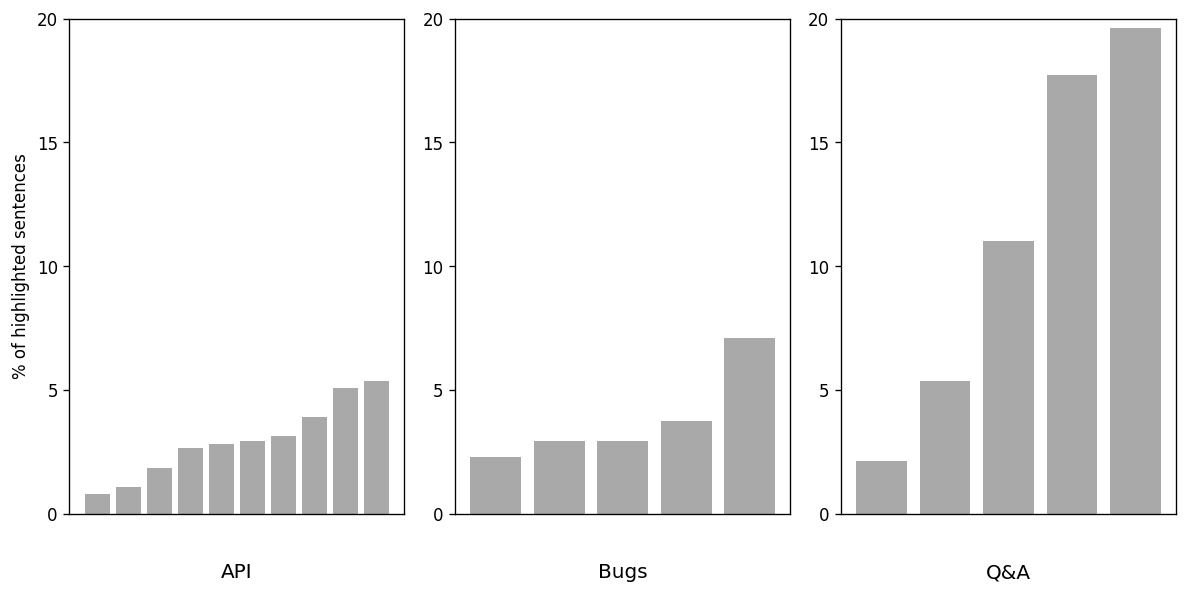
\includegraphics[width=.98\textwidth]{cp3/task-artifact-ratio}
    \caption{Percentage of highlighted sentences per artifact grouped by artifact's type}
    \label{fig:task-artifact-ratio}
\end{figure}

\subsubsection{How much agreement is there between participants about the text relevant to a task?}
\label{cp3:agreement}


With this question, we seek to identify if there is a set of key sentences that
participants unanimously consider relevant to a task. 
We use Nenkova and Passonneau's
pyramid method~\cite{Nenkova2004}
to investigate the degree to which participants agree upon
the text relevant to a task. This method was originally used
to quantify the content of summaries produced by different annotators.
The more annotators who include the same content in their summaries,
the more consistent the view of information relevant to a summary and
the more weight is given to the selected content. We apply the same rationale
to assess the level of agreement of which HUs are relevant to a task
and whether agreement relates to how correctly
a participant completes a task.




% To construct the pyramid, we assign a weight to each HU
% corresponding to the number of participants who highlighted that HU during
% a task.
% From the 602 HUs, we observe that 18\% of them are considered relevant by eight or more participants while 58\% are relevant to only one or two participants.
Figure~\ref{fig:highlights-distribution} shows the distribution of HUs over the pyramid we produce using the pyramid method.
To facilitate interpreting the results,
we take into consideration how other studies provide categories for the relevance of
text (i.e.,~\cite{Petrosyan2015} and~\cite{Jiang2017}) and 
we aggregate HUs selected by a range of participants into three tiers.
Table~\ref{tbl:task-hu} presents HUs per tier.
Starting from the bottom tier, the pyramid represents the perceived relevance of information from less to more relevant.


We use the aggregated data (Table~\ref{tbl:task-hu}) to test if the number of HUs identified at each tier affects how correct were the solutions provided by the participants (as measured by the questionnaires applied for each task). 
Since we have three independent variables (i.e., tiers) and one outcome variable (i.e., scores),
we use a multivariate analysis of variance to test this hypothesis~\cite{wohlin2012}. 
Results indicate a significant differences ($p\text{-value} < 0.01$) between participants' score and their HUs.
We then conducted univariate tests on each tier,
finding that 
the number of HUs identified at the mid and top-tiers 
positively affect the correctness of a participant's questionnaire answer, 
suggesting that HUs from these two tiers contain key
information for completing a task.
As expected, HUs at the bottom tier vary more per participant.
Due to such variability, there is no clear indication
that bottom tier HUs are from participants from a certain group, such as all those
unfamiliar with a particular technology or  who successfully
completed a task and those who did not (Section~\ref{cp3:threats} details threats for this analysis).







\begin{figure}
    \centering
    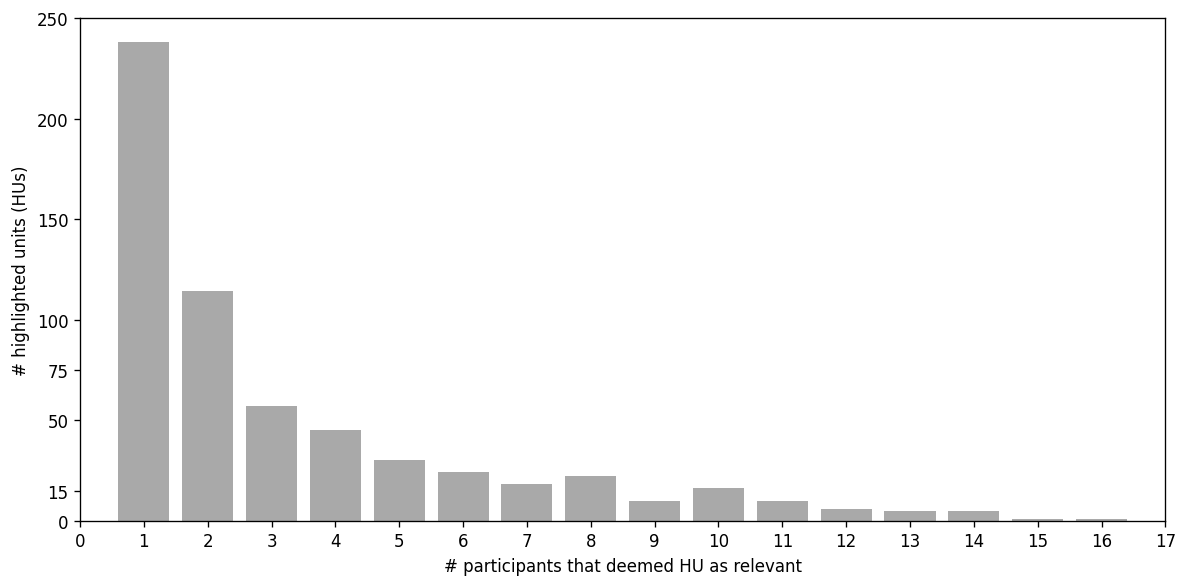
\includegraphics[width=.95\textwidth]{cp3/highlights-distribution}
    \caption{Distribution of the number of participants who deem an HU as relevant}
    \label{fig:highlights-distribution}
\end{figure}




\begin{table}
\begin{center}
\caption{Distribution of highlights and their respective percentages per tier for every task}
\begin{small}
% \vspace{-3mm}       
\begin{threeparttable} 
\rowcolors{2}{}{lightgray}
\begin{tabular}{l|c|cc|cc|cc}
\hline    
% Header
\textbf{Task}  
& \textbf{\# HUs} 
& \multicolumn{2}{c|}{\textbf{bottom tier}\tnote{\dag}} 
& \multicolumn{2}{c|}{\textbf{mid tier}\tnote{\dag}} 
& \multicolumn{2}{c}{\textbf{top tier}\tnote{\dag}}\\
\hline    
\hline

Gpmdpu & 43 & 23 & (53\%) & 10 & (23\%) & 10 & (23\%) \\     
Bugzilla & 103 & 51 & (50\%) & 22 & (21\%) & 30 & (29\%) \\
Yargs & 74 & 59 & (80\%) & 12 & (16\%) & 3 & (4\%) \\
Lucene & 95 & 54 & (57\%) & 24 & (25\%) & 17 & (18\%) \\
Databases & 159 & 84 & (53\%) & 41 & (26\%) & 34 & (21\%) \\
Networking & 128 & 81 & (63\%) & 37 & (29\%) & 10 & (8\%) \\
\hline    
\hline 
\rowcolor{white}
Total & 602 & 352 & 58\% & 146 & 24\% & 104 & 17\% \\

\hline 
\end{tabular}
\begin{tablenotes}
    \item[\dag] {\scriptsize The bottom tier includes HUs highlighted by 0--2 participants
    the mid tier includes HUs highlighted by 3--7 participants, and the top tier includes HUs highlight by at least 8 participants.}    
\end{tablenotes}   
\end{threeparttable} 
\end{small}
\label{tbl:task-hu}
\end{center}
\end{table}
    



\rev{When we consider variations in the portion of the text deemed relevant (\textit{RQ1}), we find that:}


\medskip
\begin{bluequote}
    \textit{Text perceived as relevant by more participants likely relates
    to key information for completing a task whereas information
    highlighted by a few participants may be more dependent on the knowledge of individuals.}
\end{bluequote}


\subsection{Textual Evaluation}


We examine syntactic and semantic properties 
of the highlighted text so that 
we might identify
common cues to the relevancy of text to a task (\textit{RQ2}).
Since we intend to use these cues 
in the design general technique, 
we examine the text across 
all the kinds of artifacts 
available for all the tasks. 




For our syntactic analysis,
we start by inspecting the elements that compose a sentence (i.e., nouns and verbs)
using the Python NLTK API\footnote{https://www.nltk.org/} with the CoNLL-2000 corpus~\cite{Conll2000} to automatically extract such data.
We then analyze possible patterns that may arise from the syntactic structure of the text~\cite{Robillard2015}
as well as the syntatic dependencies between verbs and  other elements related to them~\cite{Chaparro2017}, investigating if the extracted entities co-occur in multiple HUs. 
For instance, consider the sentence:
``\textit{you can use include\_fields if you want specific field names}''.
We can extract the elements dependent upon the the verb `\textit{use}' (i.e., {\small \texttt{[nsubject, use, code\_word]}})
and, if we observe that these elements co-occur in multiple HUs, we flag the pattern as a cue to the relevancy of the text.





As for semantics, we
analyze HUs for \textit{semantic
frames}~\cite{fillmore1976frame}
using frame semantic parsing~\cite{Baker1998, jurafsky2014speech}.
Semantic frames are centered around events, capturing both the event
as well as relationships, entities or participants related to that
event~\cite{fillmore1976frame, Baker1998frame}. 
We explain semantic frames by considering the application
of semantic parsing to two distinct sentences extracted 
from the \texttt{Databases} and the \texttt{Lucence} tasks, respectively.
For each sentence, Figure~\ref{fig:frame-examples} shows an
excerpt of the frame analysis for the sentences. 
The frames of each sentence (in grey) represent a triggering event and the frame elements \textit{(fe)} (in red) are arguments needed to understand the event. The enclosing square brackets mark all lexical units, or words, associated with either a frame or a frame element.

\medskip




% \begin{figure}[h!]
% \fbox{%
% \parbox{0.49\textwidth}{%
% }}
% \label{sec:frames-lucene}
% \end{figure}


\begin{figure}
\begin{mdframed}
\begin{scriptsize}
\noindent \textbf{Databases:} \textit{I have yet to see a situation where hibernate was the reason for poor performance in production.}
{\ttfamily% 
\begin{enumerate}[itemindent=0.5em,leftmargin=0.5em]
\item[] $\big[$I$\big]$\textsubscript{\color{rufous} \textbf{fe:perceiver}} have yet to $\big[$see$\big]$\textsubscript{\hl{\textbf{perception of experience}}} 

\item[] $\big[$a situation where hibernate was the reason for \dots$\big]$\textsubscript{\color{rufous} \textbf{fe:phenomenon}}
\end{enumerate}
}%

\smallskip
\noindent \textbf{Lucence:} \textit{As far as I understand that sums up totalTermFreqs for all terms of a field}
{\ttfamily% 
\begin{enumerate}[itemindent=0.5em,leftmargin=0.5em]
\item[] As far as $\big[$I$\big]$\textsubscript{\color{rufous} \textbf{fe:cognizer}} $\big[$understand$\big]$\textsubscript{\hl{\textbf{grasp}}} 

\item[] $\big[$that sums up totalTermFreqs for all terms of a field$\big]$\textsubscript{\color{rufous} \textbf{fe:phenomenon}}
\end{enumerate}
}%
\end{scriptsize}
\end{mdframed}
    \caption{Example of frames and frame elements}
    \label{fig:frame-examples}
\end{figure}


Observing the frame elements captured by the verbs \textit{see} and
\textit{understand}, both sentences have the common meaning of
describing a `\textit{phenomenon}'.
However, the frame elements
that capture the meaning of each verb differ: the former represents a
`\textit{perception of experience}' while the latter represents a
cognizer `\textit{grasp}'ing her knowledge over the 
phenomenon. 


As multiple sentences might have similar meanings,
we analyze whether there are common frame elements 
that provide cues to the relevancy of text.
For this analysis, all frame elements were extracted automatically.
We decompose HUs to obtain the semantic frames for the sentence 
using the \textit{SEMAFOR} toolkit~\cite{das2014frame}.
For a detailed definition of each frame, refer to
the FrameNet
database\footnote{https://framenet.icsi.berkeley.edu/fndrupal}.




\subsubsection{Does syntactic structure provide cues to the relevancy of text to a task?}
\label{cp3:syntactic-analysis}



We start our syntactic analysis by describing noun phrases and verb phrases
in the relevant text. 
We then describe our analysis of syntactic patterns.  



Among noun phrases, we observe that 65\% of the HUs contain acronyms or coding elements.
Existing approaches that rely on these elements to identify relevant text (e.g.,~\cite{Robillard2015} or~\cite{Jiang2016b}) would miss the remaining 35\% of the HUs in our corpus.
This value may seem acceptable at first; however there are no guarantees that
the identified 65\% HUs hold all the crucial information for task completion.
As an example, some of the HUs from the mid and topmost tiers 
do not contain obvious code words that could signal their relevancy,
such as one of the sentences in the \texttt{Bugzilla} task indicates the need for ``\textit{authentication to allow retrieving non-public data}''.
% The lack of authentication implies missing non-public data, which leads to an incomplete solution, 
% and so this sentence was considered relevant by most of the participants in our study
% even when it .





With regards to verb phrases, we observe a substantial
overlap (81\%) with verbs observed in Ko and colleagues linguistic analysis
of bug report titles~\cite{Ko2006}.
The most common verbs in the HUs include conjugations of verbs such as \textit{use}, \textit{get}, \textit{set}, \textit{be}, or \textit{do},
but with the exception of \textit{use}, \textit{get}, and \textit{set}, the
remaining top common verbs are in English stop words lists~\cite{jurafsky2014speech}. As a result, many
\acs{NLP} techniques would discard them as part of their pre-processing
steps~\cite{Bavota2016}.






As for syntactic patterns, we did not observe a large set of patterns for the variety of tasks and artifacts in our experiment,
where the prominent patterns identified (e.g., \texttt{[nsubject, do, negation]})
reflect common constructs of the English language rather than cues that we might explore for the relevancy of text.
There may be multiple explanations for these results, such as
the fact our corpus contains a small number of natural language artifacts.
Due to this reason, we also checked whether patterns from existing related work (i.e.,~\cite{Chaparro2017, Robillard2015}) applied to the text in our HUs, 
but the small number of matching patters 
raises caution on
their generalizability.



\medskip
\begin{bluequote}
    \textit{We did not find prominent syntactic cues to identify
    task-relevant information. Our analysis of highlights demonstrates:
    1) limitations of existing techniques that rely on code
    words and acronyms, 2) missed
    information that may occur due to the prevalence of verbs that
    appear in English stop word lists,
    and 3) the absence of patterns derived from the syntactic structure of
    the text.}
\end{bluequote}

 



\subsubsection{Do semantics provide cues to the relevancy of text to a task?}
\label{cp3:semantic-analysis}


We extract the frames of every HU, resulting in 3,719 frames across
the 602 HUs. Only 346 distinct frames appear across these 3,719 frames
parsed. The proportionally small number of distinct semantic frames
occurring
suggests that different HUs share frame elements. 



Table~\ref{tbl:common-frames} details the most frequent frames identified per tier, filtering to show the 
most frequent frames in a tier that have not appeared in lower tiers.
In the top-most tier, the most frequently identifying distinguishing
frames denote the \textit{cause} or \textit{likelihood} of a phenomenon.
These frames are found in sentences that explain a system's behavior, which are often crucial for task completion,
as in a sentence that provides a cause for the loss in performance when using Hibernate:
 \textit{``if you need to process lots of objects for some reason, though it can seriously affect performance}''.
Other common frames \textit{quantify relationships},
as when a sentence describes the minimum elements needed to perform an operation, e.g., \textit{``to create a flag, at least the status and the type\_id or name must be provided}''.




In the middle tier, we observe frames for actions performed by some entity (\textit{intentionally act}) or facts regarding a topic (\textit{statement}).
Other common frames relate to methods or attributes and the result of some operation such as a method call, which may be useful for identifying code related entities.
For instance, this sentence from the \texttt{Bugzilla} tasks contains both the \textit{being returned} and the \textit{fields} frame, 
\textit{``You can specify to only return custom fields by specifying \texttt{\_custom} or the field name in \texttt{include\_fields}''}.





\begin{landscape}


\begin{table}
\caption{Most common semantic meanings across all the HUs; frames are presented per tier, from the topmost tier to the bottom tier} 
\begin{scriptsize}
\vspace{-1mm}  
\begin{threeparttable}    
\begin{tabular}{|l|lclr|}

\cline{2-5}       
% 
\multicolumn{1}{c|}{} &
\textbf{Frame} &
\textbf{Freq} &
\textbf{Description} & 
\parbox[l][.4cm][c]{9.8cm}{\textbf{Example}}

\\ \hline

&
\cellcolor{lightgray} Likelihood &
\cellcolor{lightgray} 8\% & 
\parbox[l][1.2cm][c]{4.4cm}{\cellcolor{lightgray} Denotes the likelihood of a hypothetical event occurring}  &
\parbox[l][1.2cm][c]{9.8cm}{\cellcolor{lightgray} \texttt{However, it can be overkill for some types of application, and the backend \underline{could be easier} to implement with a protocol such as SSE.}} \\

\multirow{-2}{*}{\rotatebox[origin=l]{90}{\textbf{top tier}}} &
Causation &
8\% & 
\parbox[l][.8cm][c]{4.4cm}{An effect is observable due to a cause} &
\parbox[l][.8cm][c]{9.8cm}{\texttt{By default this is true, \underline{meaning} overlap tokens do not count when computing norms. }} \\

&
\parbox[l][.8cm][c]{1cm}{\cellcolor{lightgray} Relational \\ Quantity} &
\cellcolor{lightgray} 7\% & 
\parbox[l][.8cm][c]{4.4cm}{\cellcolor{lightgray} Denotes a quantifiable relationship between any two dependent entities}  &
\parbox[l][.8cm][c]{9.8cm}{\cellcolor{lightgray} \texttt{It is \underline{much faster} to get to something working with Hibernate \underline{than it is} with JDBC }} \\

\hline
\hline

&
\parbox[l][.8cm][c]{1cm}{Statement} &
12\% & 
\parbox[l][.8cm][c]{4.4cm}{Verbs and nouns that communicate the act of a speaker to address a message } &
\parbox[l][.8cm][c]{9.8cm}{\texttt{Custom fields \underline{are} normally returned by default unless this is added to exclude\_fields }} \\

\multirow{3}{*}{\rotatebox[origin=l]{90}{\textbf{mid tier}}} &
\parbox[l][.8cm][c]{1cm}{\cellcolor{lightgray} Intentionally \\ act} &
\cellcolor{lightgray} 11\% & 
\parbox[l][.8cm][c]{4.4cm}{\cellcolor{lightgray} An act performed by an entity} &
\parbox[l][.8cm][c]{9.8cm}{\cellcolor{lightgray} \texttt{The data field could, of course, have any string data; \underline{it doesn't have to be} JSON. }} \\

&
\parbox[l][.8cm][c]{1cm}{Fields\tnote{\dag}} &
11\% & 
\parbox[l][.8cm][c]{4.4cm}{Denotes mentioning an object attribute or field} &
\parbox[l][.8cm][c]{9.8cm}{\texttt{computeNorm(FieldInvert state) - computes the normalization value
for a \underline{field} }} \\

&
\parbox[l][.8cm][c]{1cm}{\cellcolor{lightgray} Being \\ returned\tnote{\dag}} &
\cellcolor{lightgray} 11\% & 
\parbox[l][.8cm][c]{4.4cm}{\cellcolor{lightgray} Denotes results from a particular operation or method call} &
\parbox[l][.8cm][c]{9.8cm}{\cellcolor{lightgray} \texttt{You need to be aware of this behaviour otherwise \underline{you will get} cryptic errors}} \\

\hline
\hline

\multirow{3}{*}{\rotatebox[origin=r]{90}{\textbf{bottom tier}}} &
Using &
17\% & 
\parbox[l][.8cm][c]{4.4cm}{An agent uses an instrument in order to achieve a purpose} &
\parbox[l][.8cm][c]{9.8cm}{\texttt{By \underline{using JDBC}, resource leaks and data inconsistency happens as work is done by the developer.}} \\

&
\cellcolor{lightgray} Purpose &
\cellcolor{lightgray} 15\% & 
\parbox[l][.8cm][c]{4.4cm}{\cellcolor{lightgray} Denotes a goal or target to be achieved} & 
\parbox[l][.8cm][c]{9.8cm}{\cellcolor{lightgray} \texttt{Object Relational Mapping \underline{empowers the use of} ``Rich Domain Object'' which are Java classes}} \\

&
Capability & 
14\%  & 
\parbox[l][.8cm][c]{4.4cm}{An entity does or does not meet the pre-conditions for some event or action} & 
\parbox[l][.8cm][c]{9.8cm}{\texttt{\underline{Can't} detect anything outside letters, arrows, ctrl, alt and shift}} \\

\hline

\end{tabular}
\begin{tablenotes}
    \item[\dag] \scriptsize Frame name was modified because its semantic meaning is specific to software engineering;    
\end{tablenotes}
\end{threeparttable}    
\end{scriptsize}
\label{tbl:common-frames}
\end{table}
\end{landscape}


The bottom tier contains frames that are common to all HUs.
The most frequent frame in the bottom tier has a semantic meaning of \textit{using}.
HUs with this frame are often sentences detailing how to use a method or a
framework to achieve some goal, what might also explain the second most frequently occurring frame, i.e., \textit{purpose}, which denotes an achievable goal. 
These two frames could be used to filter sentences that contain the means
to use a technology or API with certain intention, as this sentence explaining usage scenarios for
WebSocket and Server-Sent Events in the \texttt{Networking} task:
``\textit{One is synchronous and could/would be used for near real-time data xfer, whereas the other is asynchronous and would serve an entirely different purpose}''.





To further characterize  frame elements, 
we pairwise compare their frequency in relevant text (i.e., HUs) and non-relevant text.
Figure~\ref{fig:frame-distribution} provides insight in the distribution of frames across relevant and non-relevant sentences.
We perform a Wilcoxon signed-rank test~\cite{wohlin2012} over the distribution of frames in our data and we observe with statistical significance ($p\text{-value} \le 0.05$) 
that certain frames are more prominent in relevant or non-relevant sentences.
For example, frames that represent a \textit{required} event
are more prominent in the relevant text
as found in a sentence in the \texttt{Bugzilla} REST API that describes
how to circumvent errors due to invalid tokens:
``\textit{An error is thrown if you pass an invalid token; you will need to log in again to get a new token}''.
On the other hand, frames that relate to user discussions and that do not draw conclusions or provide 
facts about an API or technology, such as \textit{point of dispute} or \textit{reasoning} are often found in non-relevant text,
as when users discuss community's procedures in the \texttt{GPMDPU} task: ``\textit{Open a new issue following the template so we can have more details on your device}''. 




\begin{figure}
\centering
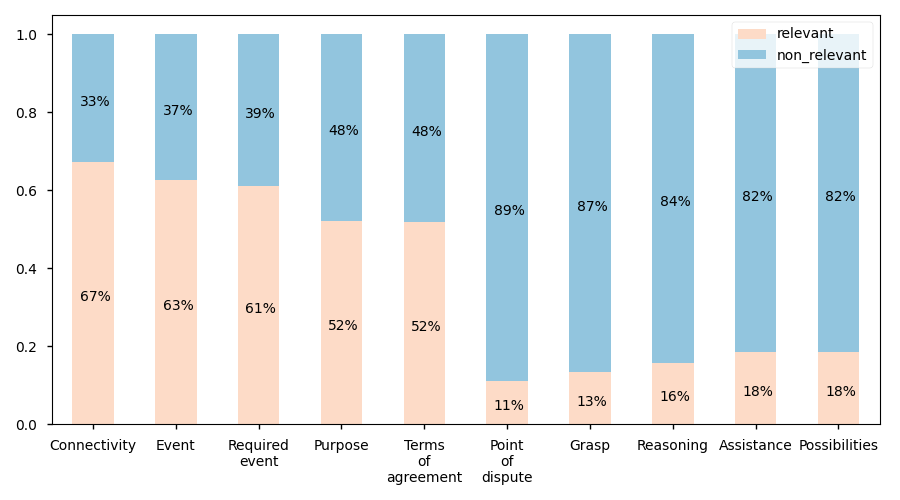
\includegraphics[width=.95\textwidth]{cp3/frames-dist-all}
\caption{Distribuion of semantic frames over the text; the figure depicts the top five frames most commonly observed in relevant and non-relevant sentences, respectively}
\label{fig:frame-distribution}
\end{figure}


While certain frames are not indicative of relevance when found on their own, we also observe that the co-ocurrance of certain frames in a sentence increase the likelihood of the sentence's relevancy.
For instance, \textit{purpose} and \textit{using} occur almost evenly across relevant and non-relevant text
while their co-occurrance is more frequent in relevant text. 
Figure~\ref{fig:frame-co-occurrence} shows the most frequent frames that co-occur and their ratio on relevant and non-relevant text.



\begin{figure}
\centering
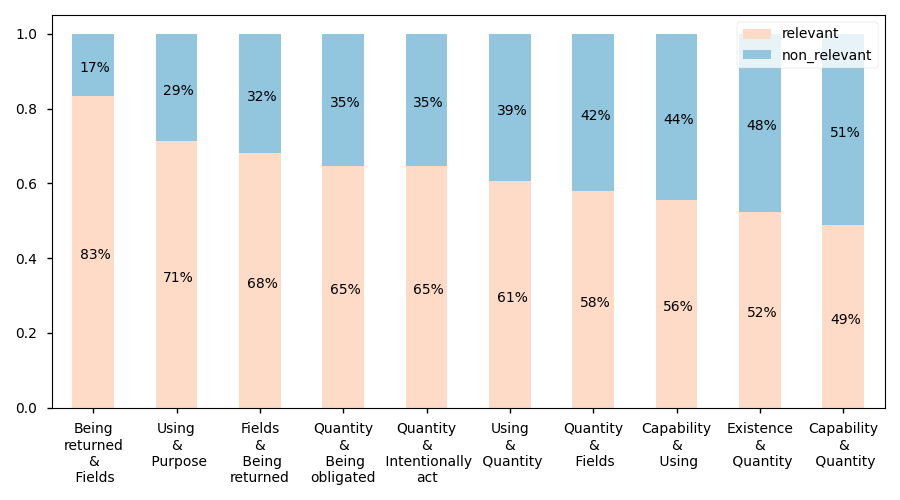
\includegraphics[width=.95\textwidth]{cp3/frames-dist-2-grams}
\caption{Distribution of co-occurring frames over the text}
\label{fig:frame-co-occurrence}
\end{figure}


Our analysis on the semantics of relevant text indicates that there exists some common aspect to the different sentences deemed as relevant.


\medskip
\begin{bluequote}
    \textit{There are recurring semantic meanings in relevant sentences,
    suggesting commonalities in their conveyed information
    and indicating that text might be identified through its semantics.}
\end{bluequote}


\subsection{Interview Analysis}

To understand how participants identified relevant text (\textit{RQ3}), we analyzed the participants'
interview responses using a card-sorting approach~\cite{spencer2009sorting}.
We\footnote{The first two authors of~\cite{marques2020}: A. Marques and N. C. Bradley} created index cards containing the interview questions and the participants' responses.
The cards were sorted into meaningful themes and then grouped into abstract categories.
We refined themes over three iterations of the data.
At each  iteration, we grouped cards containing responses on similar topics, analyzed the emerging theme, and evaluated
whether there was a broader theme that incorporated two or more of the existing themes.
To reduce individual bias, the researchers involved in this analysis independently annotated a subset of the cards at every iteration.
Disagreements occurred when more than one theme could apply to a sentence.
The annotators discussed and resolved disagreements refining the set of themes in a subsequent iteration, reaching substantial agreement ($\kappa=0.82$).





From participants' comments, we identified nine themes that we group under two major categories.
Table~\ref{tbl:themes-categories} details observed categories, themes, and the number of participants who made a comment pertaining to that theme.
We discuss results per category illustrating comments that best exemplify a theme. To facilitate the discussion we highlight themes (in gray)
when we first mention them.



% This analysis led us to a final set of nine themes (Table~\ref{tbl:themes-categories}). We discuss these themes (grey highlights) grouping them under two major categories: \textit{Search strategies} and \textit{Search challenges}.


\afterpage{

\begin{table*}[t]
\caption{Key themes relating to developers' assessment of relevancy}
\begin{scriptsize}
% \vspace{-3mm}        
\begin{threeparttable}    
\begin{tabular}{|l|llr|}

\cline{2-4}        

\multicolumn{1}{c|}{} 
& \parbox[l][.4cm][c]{2.3cm}{\textbf{Theme}}
& \textbf{Definition}
& \textbf{\#}

\\ \hline

\multirow{5}{*}{\rotatebox[origin=r]{90}{\textbf{Searching Strategy}}} 
& \parbox[l][1.7cm][c]{2.3cm}{\cellcolor{lightgray} document-guided}
& \parbox[l][1.7cm][c]{8cm}{\cellcolor{lightgray} Knowledge about the structure of the document influences how a developer locates relevant text in that particular document, e.g., the fact that StackOverflow has accepted answers, or that bug reports might have status changes such as when a user closes a bug marking it as resolved} 
& \cellcolor{lightgray} 15 \\


 
& \parbox[l][.5cm][c]{2.3cm}{ keyword-matching} 
& \parbox[l][.5cm][c]{8cm}{ The use of keywords and search filters to locate relevant text} 
&  13 \\


& \parbox[l][1.2cm][c]{2.3cm}{\cellcolor{lightgray} skimming} 
& \parbox[l][1.2cm][c]{8cm}{\cellcolor{lightgray} The act of quickly reading a portion of a document to locate relevant text. It also represents the act of scrolling from a document's sections and deciding to stop at certain points}
& \cellcolor{lightgray} 11 \\

 
& \parbox[l][.4cm][c]{2.3cm}{ scrutinizing}
& \parbox[l][.4cm][c]{8cm}{ The act of carefully reading a document/section due to some reason}
&  10 \\

 
& \parbox[l][.9cm][c]{2.3cm}{\cellcolor{lightgray} summarizing}
& \parbox[l][.9cm][c]{8cm}{\cellcolor{lightgray} The desire to first have an overview of a document or section's content before deciding which portions are worth investigating}
& \cellcolor{lightgray} 9 \\


\hline
\hline

\multirow{4}{*}{\rotatebox[origin=r]{90}{\textbf{Challenges}}}
& \parbox[l][.9cm][c]{2.3cm}{ missed-information} 
& \parbox[l][.9cm][c]{8cm}{ Acknowledgement that some information deemed relevant was missed due to the developer's search strategy} 
&  11 \\

& \parbox[l][.9cm][c]{2.3cm}{\cellcolor{lightgray} familiarity}
& \parbox[l][.9cm][c]{8cm}{\cellcolor{lightgray} How familiar is a developer with the domain of the task and/or technology and how his expertise affects her foraging process} 
& \cellcolor{lightgray} 10 \\

&  \parbox[l][.9cm][c]{2.3cm}{statement-checking} 
& \parbox[l][.9cm][c]{8cm}{ The text contains facts that are not accurate and information might be ambiguous or contradictory} 
&  7 \\

& \parbox[l][.5cm][c]{2.3cm}{\cellcolor{lightgray} verbosity} 
& \parbox[l][.5cm][c]{8cm}{\cellcolor{lightgray} The structure of the text is verbose or extensive hindering readability} 
& \cellcolor{lightgray} 5 \\

\hline

\end{tabular}
\begin{tablenotes}\scriptsize
    \item[\#] Indicates number of participants who have quotes related to the theme.
\end{tablenotes}
\end{threeparttable}    
\end{scriptsize}
\label{tbl:themes-categories}
\end{table*}

}



\subsubsection{How do developers locate relevant information?}
\label{cp3:search-strategies}

Developers often use a mix of \hl{\textit{keyword-matching}} and \hl{\textit{skimming}}~\cite{Starke2009, Ko2006a} to find relevant information within an artifact. 
Some participants said they use these search strategies for all types of artifacts, while others said they use knowledge of a document's structure to assist their searches (\hl{\textit{document-guided}}).


% \pquote{}{P12} \medbreak

\smallskip
% \begin{footnotesize}
\begin{quote}
    ``\textit{Definitively [my strategy] wasn't always the same. Going through a StackOverflow question, I would obviously read the first response. For API docs, keywords were the go to. Bug reports are hard. Comments are ordered chronologically and the first ones are sometimes not the most relevant ones}''---P12
\end{quote}
% \end{footnotesize}


Participants were also aware of the shortcomings of some artifact types and were less willing to use faster but less accurate strategies like skimming or keyword-matching for these artifacts when the tasks were difficult. 
In these cases, participants mentioned that they used a \hl{\textit{scrutnizing}} strategy:


\smallskip
% \begin{footnotesize}
\begin{quote}
    ``\textit{I usually read every comment [on StackOverflow]. Obviously, they are ranked, but, in general, every single comment could have something important}''---P11
\end{quote}
% \end{footnotesize}
    


Regardless of strategy, participants mentioned using 
implicit criteria to decide when to (not) read some text.
Such implicit criteria often relate to information foraging theory (Section~\ref{cp2:searching}) and how an individual follows some
\hl{\textit{information scent}} for judging the cost of investigating some text according to available cues~\cite{Pirolli1999}, such as the presence of bullet-points, bold text, or the conciseness and readablilty of the text.



\subsubsection{What challenges do developers face while searching for relevant information?}
\label{cp3:search-challenges}


Participants also commented on factors that made assessing the relevancy of text difficult.
The most common challenge was \hl{\textit{missing information}} that other participants deemed relevant.



\smallskip
% \begin{footnotesize}
\begin{quote}
    ``\textit{This [highlight] is a valid alternative if you don't want to use the conflicts [method]. I basically didn't see this because of how I was searching}''---P2
\end{quote}
% \end{footnotesize}




We consider missing relevant information as a major threat to task completion because it can lead to an incomplete or incorrect solution~\cite{Murphy2005};
usually, participants missed information due to their workflows, as \textit{P15} explains:





\smallskip
% \begin{footnotesize}
\begin{quote}
    ``\textit{It's hard to say that I would have picked [those highlights] without being directed to that. I believe that I knew that there were specific questions coming, but even if I was doing it for myself, I would probably skim first and then, when I start to code, it would be a natural thing to get back and dive into the details}''---P15
\end{quote}
% \end{footnotesize}



Participants also missed information due to text \hl{\textit{verbosity}}. 
Bloated text makes it harder for developers to locate task-relevant information~\cite{robillard2011field} as it is more cognitively demanding to read verbose text:


\smallskip
% \begin{footnotesize}
\begin{quote}
    ``\textit{When I looked at the API documentation, there was too much text. I was mentally exhausted just looking at it}''---P6
\end{quote}
% \end{footnotesize}


Participants noted that their \hl{\textit{familiarity}} with the task domain also affected how they located relevant information in the text.



\smallskip
% \begin{footnotesize}
\begin{quote}
    ``\textit{The easiest one was the one about ORM/JDBC [databases] because I was so familiar with these technologies}''---P2
\end{quote}
% \end{footnotesize}




Finally, when presented with \hl{\textit{ambiguous or contradictory}} information, participants had to spend time seeking out additional information to resolve the ambiguity.


\smallskip
% \begin{footnotesize}
\begin{quote}
    ``\textit{I think it was in this one [highlight]. They said that \texttt{cmd} works in the same way as \texttt{Ctrl}, but I went with the one that says otherwise. [...] it was actually helpful to have two other highlights so I had a bit more reliance on the thing that was mentioned by more users.}''---P19
\end{quote}
% \end{footnotesize}



Our analysis on the participants' comments on their search strategies provides further insights into how developers forage for information in software development natural language artifacts. One of our key observations is that  developers use mixed strategies to locate task-relevant information. In doing so, developers often miss some information that might be relevant to the task that they are performing.


\medskip
\begin{bluequote}
    \textit{Developers use mixed strategies to locate task-relevant information, often missing some information that might be relevant to complete a task completely and correctly.}
\end{bluequote}




\subsection{Summary of Results}


The results we obtained 
from the analysis of highlights produced by 
developers  indicate that
between 1\% to 20\% of the text of an artifact was considered
relevant to a task.
While we failed to observe syntactic cues 
that could indicate the relevance of text to a task, 
we observe consistency in the meaning of the relevant text---as captured using frame semantics---suggesting that semantic-based approaches 
may be more appropriate for the 
automatic identification of task-relevant text.

% inspecting artifacts 
% pertinent to six software tasks



\subsection{Threats to Validity}
\label{cp3:threats}


In this section, we discuss threats from our experimental design 
and from our
examination of the relevant text (HUs) produced by participants who 
inspected natural language artifacts from six information seeking tasks. 



The design of the six tasks in our experiment represents a threat to
\textit{construct validity}.  To mitigate this threat, we used results from studies discussing the search
behaviour of developers~\cite{umarji2008archetypal, Li2013, Xia2017} as
input to the design of our tasks.
For each task, our goal was to provide a set of artifacts so that a
participant could gather enough knowledge to complete the task, which
we confirmed through pilot studies.  The provision of artifacts was also
necessary to enable a systematic analysis of relevance through a
controlled experiment. We mitigated threats on artifact
selection by asking external researchers to provide their own list of
candidate artifacts, which was similar to our own list.



The \textit{external validity} of the experimental results is affected
by the participants, the tasks and the artifacts.  Considering the
subjective nature of relevance, the knowledge and particularities of
our participants may not generalize to other software developers.
Furthermore, the structure and linguistic characteristics of the
artifacts considered may not extend to other kinds of artifacts or the
same kind of artifacts in other domains.  We tried to mitigate this
threat by selecting different kinds of artifacts such as API
documentation, bug reports, and Q\&A pages while 
ensuring that each kind was present in at least
50\% of the tasks. 
However, our results
are bound to the domains and artifacts we evaluated and may not generalize.
Future work should confirm our findings on a wider range of artifacts and tasks.


There are also threats to the validity of our
\textit{conclusions}.
Experimental procedures encouraged participants to work on the tasks using their normal workflow.
However, at least one participant (\textit{P15}) indicated that they would normally
revisit a document as different information needs arise as part of a task.
As a result, our study may miss relevant information.
In addition, the text participants highlighted may not have always aligned with the text that contained information useful for completing the task.
To investigate this alignment further, we would have had to create an oracle containing the relevant text.
Unfortunately, creating the oracle is challenging because it would need to encompass different perceptions of relevance~\cite{Pirolli1999,saracevic1975,Nenkova2004} and usefulness~\cite{Freund2013, Freund2015}.
Thus, to avoid the subjective and imprecise process of judging alignment, we simply consider any text highlighted by participants as containing information useful to completing the tasks.



While the size of our corpus might also affect our conclusions,
we emphasize that the HUs from mid and top-tiers in our data comprise 250 sentences, 
which is similar to the amount of data studied previously. For instance, the McGill~\cite{Petrosyan2015}
and Android~\cite{Jiang2016b} datasets contain 238 and 141 relevant text fragments, respectively.


To extract the meaning of text through parsed frames, 
we used a general frame semantics database rather than one
specific to software engineering.  This led to frames that were
\textit{out-of-context}, causing us to adapt either the frame's
name or its description.  
Frames adapted to software engineering (e.g., \textit{being returned}
and \textit{fields}) represent a small fraction of all the extracted
frames. As a result, we argue that all the sentences containing them still have
similar semantic meanings and our conclusions are not
affected by these out-of-context frames. However, as we discuss in Chapter~\ref{ch:discussion}, 
having specific
software engineering frames could improve our results.




% \subsection{Summary of results}


